\begin{figure}[h]
  \begin{center}
    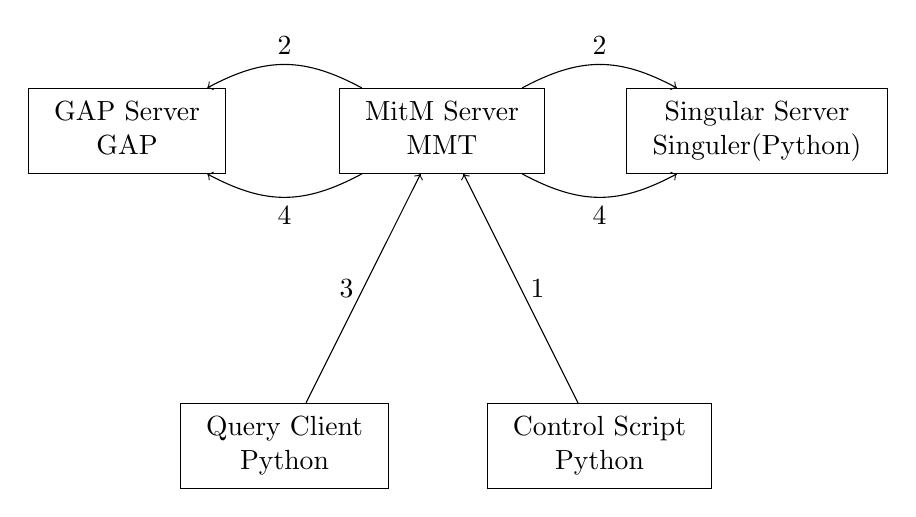
\begin{tikzpicture}[xscale=2, yscale=4]\normalsize
      \node[draw] (g) at (0,0) {
        \begin{tabular}{c}
          GAP Server \\GAP
        \end{tabular}
      };
      \node[draw] (m) at (2,0) {
        \begin{tabular}{c}
          MitM Server\\MMT
        \end{tabular}
      };
      \node[draw] (s) at (4,0) {
        \begin{tabular}{c}
          Singular Server\\Singuler(Python)
        \end{tabular}
      };
      \node[draw] (p) at (1, -1) {
        \begin{tabular}{c}
          Query Client\\Python
        \end{tabular}
      };
      \node[draw] (c) at (3, -1) {
        \begin{tabular}{c}
          Control Script\\Python
        \end{tabular}
        };
      \draw[->] (c) to node[right] {1} (m);
      \draw[->] (m) to[bend left=15] node[above] {2} (s);
      \draw[->] (m) to[bend right=15] node[above] {2} (g);
      \draw[->] (p) to node[left] {3} (m);
      \draw[->] (m) to[bend right=15] node[below] {4} (s);
      \draw[->] (m) to[bend left=15] node[below] {4} (g);
    \end{tikzpicture}
  \end{center}

  \caption[GAP-Singular MitM Interaction]{
    System Designed to Prove the Concept of the MitM Protocol
  }
  \label{fig:mitmpoc}
\end{figure}
